\documentclass[a5paper]{article}

\usepackage{amsmath, amssymb}
\usepackage{multicol}
\setlength{\columnsep}{1cm}
\usepackage[margin=0.75in]{geometry}
\usepackage{graphicx}
\graphicspath{ {../../../Images/MATH11218/} }
\usepackage[breaklinks, hidelinks]{hyperref}
\usepackage{siunitx}
\usepackage{tikz}
\usepackage{pgfplots}
\pgfplotsset{compat=newest}
\usepgfplotslibrary{external}
\usepackage{stix}
\usepackage{ragged2e}
\usepackage{enumitem}
\usepackage{polynom}

\newcommand{\sech}{\mathrm{sech}}
\newcommand{\csch}{\mathrm{csch}}

\sisetup{
	round-mode = places,
	round-precision = 2,
}

\title{MATH11218 \\ Methods and Basically Specialist Revision}
\author{Authored by: Lachlan J. W. Wyer}
\date{\today}

\begin{document}
	\maketitle
	\tableofcontents
	\pagebreak

	\section{Introduction}
	\subsection{Indices:}
	Within the expression of $a^{m}$, a is considered to be the base with the power m being the index. The reason that this is considered useful is in scientific notation to expression large numbers, or simplify repeated multiplication, fractions, roots or polynomials. E.g. $2\times 2\times 2\times 2\times 2\times 2=2^{6}$. With these there are a number of different index laws that goes with it:
	\begin{enumerate}
		\item $a^{m}\cdot a^{n}\;=\;a^{m+n}$
		\item $\frac{a^{m}}{a^{n}}\;=\;a^{m-n}$
		\item $(a^{m})^{n}\;=\;a^{m\cdot n}$
		\item $(ab)^{m}\;=\;a^{m}b^{m}$
		\item $(\frac{a}{b})^{m}\;=\;\frac{a^{m}}{b^{m}}$
		\item $a^{\frac{m}{n}}\;=\;\sqrt[n]{a^{m}}$
		\item $a^{0}\;=\;1$
	\end{enumerate}

	\subsection{Poynomials:}
	A polynomial explains/denotes the degree or curviness that a line is at. Such as a constant can be described as being degree 0, linear degree 1, quadratic degree 2, cubic degree 3 and  so on.
	\subsubsection*{Quadratics}
	With quadratics it is important to understand that it can contain multiple different types of roots. For example, iff: $\Delta=b^{2}-4ac$
	\begin{itemize}
		\item $\Delta\;>\;0$, when it contains 2 real roots, e.g. $(x+a)(x+b)$.
		\item $\Delta\;=\;0$, when there is 1 real root, e.g. $(x+a)^{2}$.
		\item $\Delta\;<\;0$, when no real roots are found, e.g $(x+aj)(x+bj)$.
	\end{itemize}
	\subsubsection*{Polynomials with Degrees Greater than 2}
	When a polynomial contains a degree that is greater than 2, it roots can be found through a process called polynomial long division.
	\medskip
	\begin{center}
		\polylongdiv{x^{3}+3x^{2}-10x-24}{x+2}\\
		\smallskip
		\begin{align*}
			\therefore\;\;x^{3}+3x^{2}-10x-24\;&=\;(x+2)(x^{2}-x-12)\\
			&=\;(x+2)(x-4)(x+3)\\
			x\;&=\;-3,\;-2,\;4
		\end{align*}
	\end{center}

	\subsection{Algebraic Functions:}
	Within fractional functions there are two main types:
	\begin{enumerate}
		\item Proper fractions, where the denominator is smaller then the numerator.
		\item Improper fractions, where the denominator is less or equal to the numerator.
	\end{enumerate}
	It is important to note, that the greater, equal to, and less than are only relative to polynomial degree. Some parts to with division of fraction is just the multiplication of the recipricol, $\frac{a}{b}\;\div\;\frac{c}{d}\;=\frac{a}{b}\;\times\;\frac{d}{c}$.
	\begin{align*}
		\frac{2}{x+1}\;+\;\frac{4}{x+2}\;&=\;0\\
		&=\;\frac{2(x+2)\;+\;4(x+1)}{(x+1)(x+2)}\\
		&=\;\frac{2x+4+4x+4}{(x+1)(x+2)}\\
		&=\;\frac{6x+8}{(x+1)(x+2)}\\
		\therefore\;\;x&\not =\;-2,\;-1
	\end{align*}

	\pagebreak

	\section{Sum Notation}
	\subsection{Inequalities:}
	\begin{align*}
		&<\;\text{- Less than}\\
		&>\;\text{- Greater than}\\
		&\leq\;\text{- Less than or equal to}\\
		&\geq\;\text{- Greater than or equal to}
	\end{align*}
	For example:
	\begin{align*}
		1\;-\;2t\;&<\;7\\
		-2t\;&<\;6\\
		t\;&>\;-3
	\end{align*}
	\smallskip
	$\frac{x}{y}\;>\;0\;\text{OR}\;xy\;>\;0$, presents two different cases in the possible solutions that it presents:
	\begin{enumerate}[start=1,label={Case \roman* - },wide = 25pt, leftmargin = 3em]
		\item $x\;\&\;y\;>\;0$
		\item $x\;\&\;y\;<\;0$
	\end{enumerate}
	\smallskip
	$\frac{x}{y}\;<\;0\;\text{OR}\;xy\;<\;0$, also presents two different cases in the possible solutions that it presents:
	\begin{enumerate}[start=1,label={Case \roman* - },wide = 25pt, leftmargin = 3em]
		\item $x\;<\;0\&\;y\;>\;0$
		\item $x\;>\;0\&\;y\;<\;0$
	\end{enumerate}

	\subsection{Partial Fractions:}
	These are used on improper fractions to complete polynomial long division.
	\smallskip
	\begin{center}
		\polylongdiv{2x^{3}+4x-1}{2x-2}
		\break\hfill\break\break
		$2x^{3}+4x-1=x^{2}+x+3+\frac{5}{2x-2}$
	\end{center}
	Some equations for the partial fractions, always assuming that the denominator is of a higher degree than the numerator:
	\begin{enumerate}
		\item $\frac{f(x)}{(x+a)(x+b)}\;=\;\frac{A}{x+a}\;+\;\frac{B}{x+b}$
		\item $\frac{g(x)}{(x+c)^{n}}\;=\;\frac{A}{x+c}\;+\;\frac{B}{(x+c)^{2}}\;+\ldots+\;\frac{Z}{(x+c)^{n}}$
		\item $\frac{h(x)}{(ax^{2}+bx+c)(x+d)}\;=\;\frac{Ax\;+\;B}{ax^{2}+bx+c}\;+\;\frac{C}{x+d}$
	\end{enumerate}
	(e.g.)
	\begin{center}
		$$\frac{2x^{4}-8x{2}+5x-2}{x^{3}-4x}$$\\
		\polylongdiv{2x^{4}-8x^{2}+5x-2}{x^{3}-4x}\\
		\begin{align*}
			\frac{2x^{4}-8x{2}+5x-2}{x^{3}-4x}&=2x+\frac{5x-2}{x^{3}-4x}\\\\
			\frac{5x-2}{x(x^{2}-4)}&=\frac{A}{x}+\frac{Bx+C}{x^{2}-4}\\
			&=\frac{A(x^{2}-4)+(Bx+C)x}{x(x^{2}-4)}\\\\
			\therefore\;\;5x-2&=A(x^{2}-4)+(Bx+C)x\\
			&=Ax^{2}-4A+Bx^{2}+Cx
		\end{align*}
	
		\begin{align*}
			x^{2} & & x^{1} & & x^{0} \\
			0&=A+B & 5&=C & -2&=-4A \\
			0&=\frac{1}{2}+B &  &  & A&= \frac{1}{2} \\
			B&=-\frac{1}{2} &  &  &  &
		\end{align*}
	\end{center}

	\pagebreak

	\section{Vectors}
	\subsection{Polar Co-ordinates:}
	Here just consider the "x" and "y" co-ordinates of a vector as just the relationship between the angle and hypotenuse.
	$$r\;<\;\theta$$
	Where:
	\begin{itemize}
		\item r is the magnitude
		\item $\theta$ is the angle, usually measured from the $x$-axis
	\end{itemize}
	As such, to find the different aspects of polar co\-ordinates use the following formulas.
	\begin{align*}
		x&=r\cos(\theta)\\
		y&=r\sin(\theta)\\\\
		r&=\sqrt{x^{2}+y^{2}}\\
		\theta&=\arctan(\frac{y}{x})\\\\
		&\text{For 3D vectors:}\\
		r&<\theta<\varphi
	\end{align*}
	
	\subsection{Vectors:}
	Remember the scene from Minions, Vector(s) need both direction \& and magnitude, $\hat{v}=\frac{\vec{v}}{\lvert v\rvert}$.
	
	\pagebreak

	\section{Engineering Functions I}
	\subsection{Number Systems:}
	Within the part of pure mathematics there are several different types of number systems:
	\begin{itemize}
		\item $\mathbb{N}$: All types of numbers. This can be further split into $\mathbb{N}^{+}\;\&\;\mathbb{N}^{-}$
		\item $\mathbb{W}$: Just the whole numbers
		\item $\mathbb{Z}$: The interger set
		\item $\mathbb{Q}$: Rational numbers, these include numbers that terminate, recurring of can be defined in a fraction
		\item $\mathbb{I}$: Irrational numbers such as $\pi$, $e$, or $\sqrt{2}$
		\item $\mathbb{R}$: Real numbers
		\item $\mathbb{C}$: Complex set
	\end{itemize}

	\subsection{The Function:}
	The function f(x), define the range [f(x)] as dependend on the domain [x]. This allows the function be restricted over a specified domain. Within functions there are several main types of functions. For a graph to be considered a function it must pass the vertical line test.
	\subsubsection{Even Function}
	These are functions that are symmetrical about the y\-axis, e.g. $f(-x)=f(x)$.
	\subsubsection{Odd Function}
	These are symmetrical about the rotation of the origin, e.g. $f(-x)=-f(x)$.
	\subsubsection{Domain}
	The domain can be specified as the set of values that can be inputed into the function. In real-world examples, physical properties, generally cannot be negative, and as such a restricted domain set must be used.
	\subsubsection{Range}
	This is just the output of the restricted set of the domain, based upon the actions that the function takes.

	\subsection{Composite Functions:}
	E.g. $f[g(x)]$. Here the range of the inner function affects the domain of the outer function.
	\begin{align*}
		f(x)&=4x+1\\
		g(x)&=2x^{2}+5x\\\\
		g[f(x)]&=2(4x+1)^{2}+5(4x+1)\\
		&=2(16x^{2}+8x+1)+(20x+5)\\
		&=32x^{2}+36x+7\\\\
		f[g(x)]&=4(2x^{2}+5x)+1\\
		&=18x^{2}+20x+1
	\end{align*}

	\pagebreak

	\section{Engineering Functions II}
	\subsection{Parametric Functions:}
	An x and y function are both affected by third variable such as distance, time or angle. For example:
	\begin{align*}
		x&=t^{2}\\
		\pm\sqrt{x}&=2\\
		y&=2t\\\\
		\therefore\;\;y&=\pm 2\sqrt{x}\\
		y&=\sqrt{2},\;\leq t\leq 5
	\end{align*}
	\subsection{Inverse Functions:}
	$y=f^{-1}(x)$ is just the line $y=f(x)$ reflected over $y=x$. An example of this is cos and arccos, $e$ and ln().

	\subsection{Break Functions:}
	\subsubsection{Continuous Functions}
	A function in where there is no break in the continuation of the function.
	\subsubsection{Piecewise Functions}
	The function contains breaks. These are points where the function might not be defined or allow joining multiple function together.
	\subsubsection{Peirodic Functions}
	This is type of function that repeats itself after a certain period. A famouns example is trigonometric functions.
	\subsubsection{Rational Functions}
	These functions are represented as fractions, $R(x)=\frac{P(x)}{Q(x)}$. It is key to note that these functions contain at least one asymptote. With the function below, @ x=-2 and x=1 it will be undefined.
	\begin{align*}
		y&=\frac{x}{x^{2}+x-2}\\
		 &=\frac{x}{(x+2)(x-1)}\\\\
		x&=-2,\;1
	\end{align*}
	\subsubsection{Modulus Function}
	This is a function where the range is always positive.
	\begin{center}
	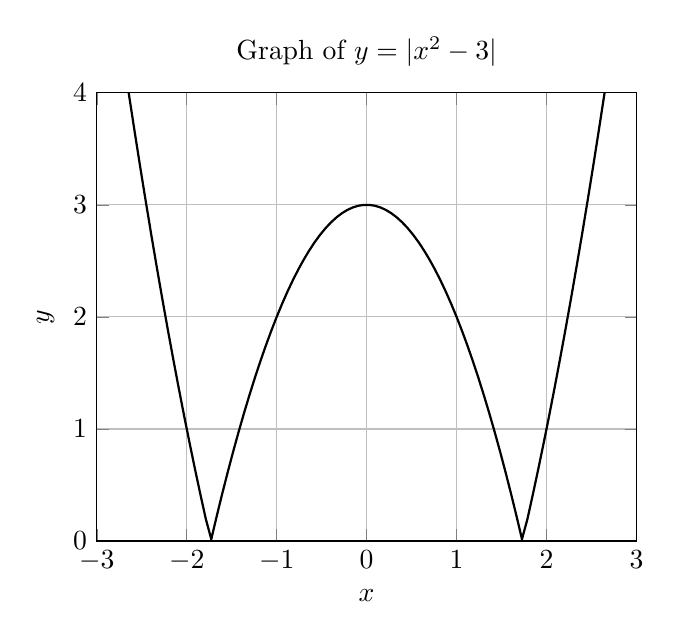
\begin{tikzpicture}
	    \begin{axis}[
		title={Graph of $ y = |x^2 - 3| $},
		xlabel={$ x $},
		ylabel={$ y $},
		grid=both,
		xmin=-3, xmax=3,
		ymin=0, ymax=4,
		domain=-3:3,
		samples=100,
		]
		\addplot[black, thick] {abs(x^2 - 3)};
	    \end{axis}
	\end{tikzpicture}
	\end{center}
	
	\subsection{Logarithms:}
	\subsubsection{Graphing}
	Log functions are the inverse of the exopential.
	$$a^{x}=b,\;log_{a}(b)=x$$
	\begin{center}
	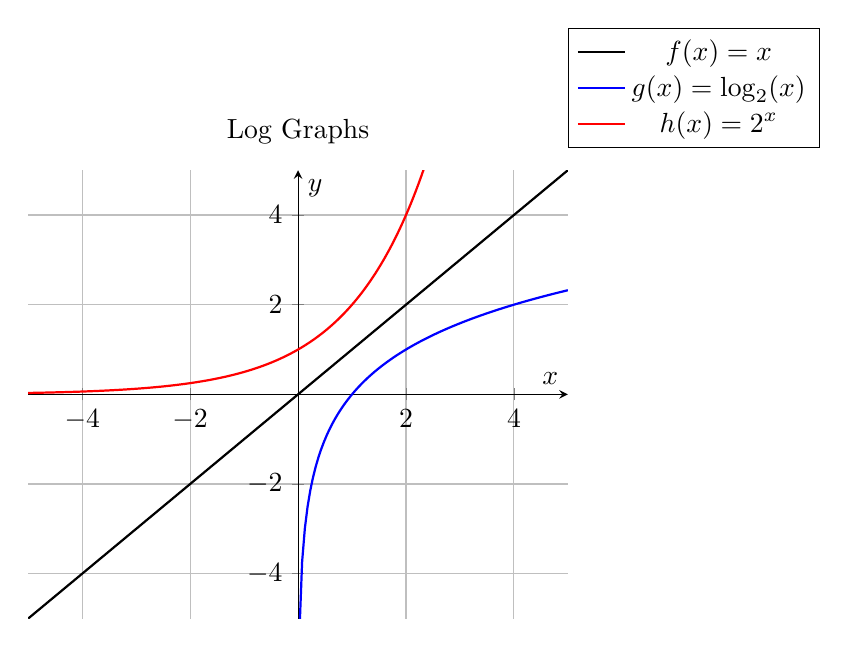
\begin{tikzpicture}
		\begin{axis}[
			title={Log Graphs},
			xlabel={$ x $},
			ylabel={$ y $},
			grid=both,
			xmin=-5, xmax=5,
			ymin=-5, ymax=5,
			domain=-5:5,
			samples=200,
			axis lines=middle,
			legend style={at={(1,1.05)}, anchor=south west},
		]
		\addplot[black, thick] {x};
		\addlegendentry{$ f(x)=x $}
		\addplot[blue, thick] {ln(x)/ln(2)};
		\addlegendentry{$ g(x)=\log_{2}(x) $}
		\addplot[red, thick] {2^x};
		\addlegendentry{$ h(x)=2^{x} $}
		\end{axis}
	\end{tikzpicture}
	\end{center}
	\subsubsection{Log Laws}
	\begin{align*}
		\log_{x}(a)+\log_{x}(b)&=\log_{x}(ab)\\
		\log_{x}(a)+\log_{x}(b)&=\log_{x}(\frac{a}{b})\\
		\log_{x}(a^{m})&=m\log_{x}(a)\\
		\log_{a}(a)&=1\\
		\log_{x}(1)&=0\\
		\log_{a}(b)&=\frac{\log_{x}(b)}{\log_{x}(a)}
	\end{align*}
	There are also some interesting properties of logs in functions, such as $a^{\log_{a}(x)}=x$ as well as $e^{\ln(x)}=x$.

	\subsection{Exponential Functions:}
	\begin{center}
	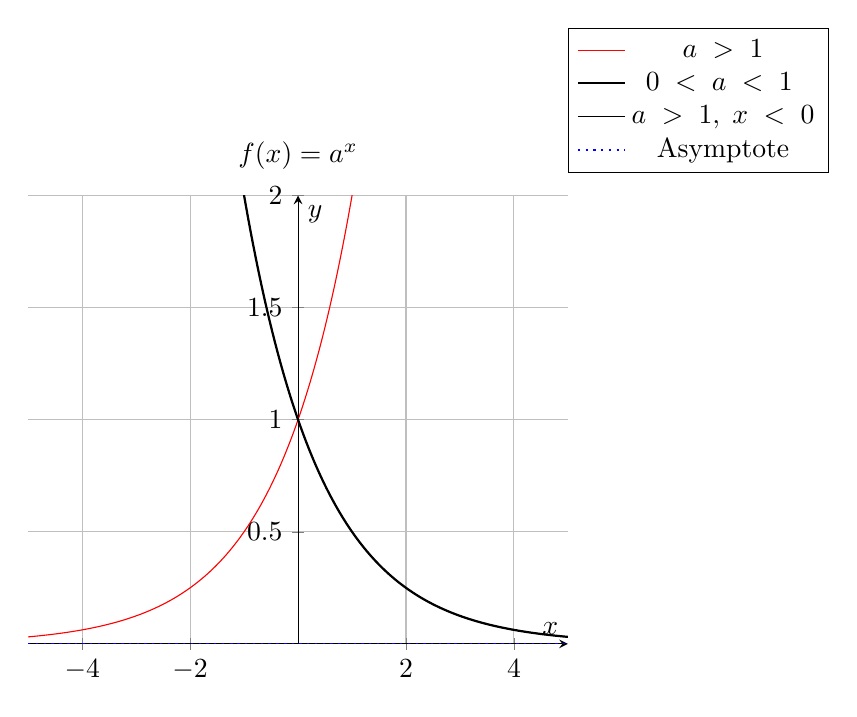
\begin{tikzpicture}
		\begin{axis}[
			title={$ f(x)=a^{x} $},
			xlabel={$ x $},
			ylabel={$ y $},
			grid=both,
			xmin=-5, xmax=5,
			ymin=0, ymax=2,
			domain=-5:5,
			samples=200,
			axis lines=middle,
			legend style={at={(1,1.05)}, anchor=south west},
		]
		\addplot[red] {2^x};
		\addlegendentry{$ a\;>\;1 $}
		\addplot[black, thick] {0.5^x};
		\addlegendentry{$ 0\;<\;a\;<\;1\; $}
		\addplot[black] {0.5^x};
		\addlegendentry{$ a\;>\;1,\;x\;<\;0 $}
		\addplot[dotted, blue, thick] {0};
		\addlegendentry{ Asymptote }
		\end{axis}
	\end{tikzpicture}
	\end{center}

	\subsection{Hyperbolic Functions:}
	\begin{center}
		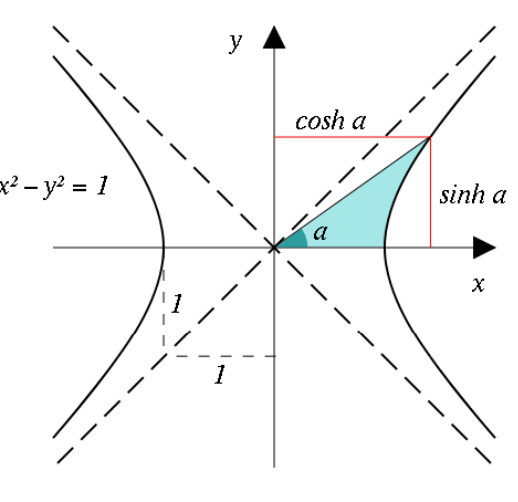
\includegraphics[scale=0.75]{hyperbolic-func.png}
	\end{center}
	\begin{align*}
		\sinh(x)&=\frac{e^{x}-e^{-x}}{2} & \csch(x)&=\frac{2}{e^{x}-e^{-x}}\\
		\cosh(x)&=\frac{e^{x}+e^{-x}}{2} & \sech(x)&=\frac{2}{e^{x}+e^{-x}}\\
		\tanh(x)&=\frac{\sinh(x)}{\cosh(x)} & \coth(x)&=\frac{e^{x}+e^{-x}}{e^{x}-e^{-x}}\\
		&=\frac{e^{x}-e^{-x}}{e^{x}+e^{-x}} & 
	\end{align*}
	\subsubsection{Hyperbolic Identities}
	\begin{align*}
		\sinh(-x)&=-\sinh(x)\\
		\cosh(-x)&=\cosh(x)\\\\
		\cosh^{2}(x)-\sinh^{2}(x)&=1\\
		1-\tanh^{2}(x)&=\sech^{2}(x)\\
		\coth^{2}(x)-1&=\csch^{2}(x)\\\\
		\sinh(x\pm y)&=\sinh(x)\cosh(y)\pm\cosh(x)\sinh(y)\\
		\cosh(x\pm y)&=\cosh(x)\cosh(y)\pm\sinh(x)\sinh)y)\\\\
		\sinh(2x)&=2\sinh(x)\cosh(x)\\
		\cosh(2x)&=\cosh^{2}(x)+\sinh^{2}(x)\\\\
		2\cosh^{2}(x)&=\cosh(2x)+1\\
		2\sinh^{2}(x)&=\cosh(2x)-1\\\\
		e^{x}&=\cosh(x)+\sinh(x)\\
		e^{-x}&=\cosh(x)-\sinh(x)
	\end{align*}
\end{document}
